% Data augmentation for the Phase 2 U-Net (Piyush)
% Code: src/dl_augment.py (python -m src.dl_augment runs the self-check), flag --aug in src/train_dl.py.
% Numbers come from reports/dl/checks/aug_ablation.csv and aug_ablation_diffs.csv (python -m src.dl_aug_report --boot).

\section{Data Augmentation}
\label{sec:dl_aug}

A fire spreads the same way whether the map is turned or mirrored, as long as the wind turns with it. Flips
and 90-degree rotations therefore give new, physically valid training patches for free, and they are a
standard way to make segmentation networks generalise from few examples~\cite{ronneberger2015}. We test
whether they help the focal U-Net.

\textbf{Transforms.} Each training patch receives one transform drawn at random from a set: \texttt{flip}
(identity, left-right, up-down, both), \texttt{rot} (0, 90, 180, 270 degrees) or \texttt{flip\_rot} (all
eight symmetries of the square). The same transform is applied to all 12 input channels and to the label,
so pixels labelled $-1$ stay masked. Eval and test patches are never transformed.

\textbf{Turning the wind.} Moving the pixels is not enough. The channel \texttt{th} is the direction the
wind blows \emph{from}, in degrees clockwise from north, and it is a number, not a direction in the image. If a
patch is rotated but \texttt{th} is not, the fire spreads in a direction the wind no longer points to, and
the model is taught wrong physics. Let $s=+1$ if the row index grows northward and $s=-1$ if it grows
southward. Then
\begin{align}
\text{left-right flip:}\quad & \theta \mapsto -\theta \pmod{360}, \nonumber\\
\text{up-down flip:}\quad & \theta \mapsto 180 - \theta \pmod{360}, \label{eq:aug_th}\\
\text{rotation by } k \times 90^\circ\text{:}\quad & \theta \mapsto \theta + 90\,k\,s \pmod{360}, \nonumber
\end{align}
where the rotation is \texttt{torch.rot90} with $k$ quarter turns from the row axis towards the column axis.
The flips do not depend on the grid orientation, but the rotation does. The patches are stored
south-up (Section~\ref{sec:method}), so $s=+1$: \texttt{rot90} sends a pixel offset (row, column) to
($-$column, row), which takes east to south, a clockwise turn on the map, and the bearing grows by
$90^\circ$. On a north-up grid the same call would turn the map anticlockwise. The loaders hold
z-scored data, so \texttt{th} is converted back to degrees with the training mean and standard deviation,
turned, wrapped to $[0, 360)$ and z-scored again. It is not clipped again to the training 0.5--99.5
percentile range (10 to 339 degrees): that clip removes export errors, but a valid turned angle such as
5 degrees falls outside it.

\textbf{Check.} The self-check builds a patch with a known wind direction and puts its next-day fire 12\,km
downwind of the centre. For all eight transforms and five wind directions it checks that after the transform
the fire is still downwind of the new \texttt{th}, that the label moves with the input, and that a
90-degree turn adds $90^\circ$. Run with the opposite rotation sign, or with \texttt{th} left unturned, the
check fails.

\textbf{Runs.} We trained the focal U-Net with \texttt{-{}-aug} set to \texttt{none}, \texttt{flip},
\texttt{rot} and \texttt{flip\_rot}, each with seeds 0, 1 and 2; everything else is as in the loss sweep
(Section~\ref{sec:dl_loss}). To measure whether turning the wind matters, one more run uses
\texttt{flip\_rot} with \texttt{th} deliberately left unturned. All 13 runs used the same machine, an Apple
M3 GPU, because a same-seed rerun alone moves test PR AUC by up to 0.02 (Section~\ref{sec:dl_validation}),
so we do not compare against the T4 runs of the loss sweep. The rule was fixed before the runs: the mode with
the highest mean eval PR AUC is used for the final U-Net, and \texttt{none} stays unless that mode beats it
by more than one seed standard deviation.

\begin{table}[t]
\centering
\caption{Augmentation for the focal U-Net: mean $\pm$ standard deviation over seeds 0, 1 and 2 (the
run with \texttt{th} not turned has seed 0 only). Eval PR AUC (best epoch) decides; the test columns are
reported only. All runs on one Apple M3 GPU.}
\label{tab:dl_aug}
\footnotesize
\setlength{\tabcolsep}{2.6pt}
\renewcommand{\arraystretch}{1.12}
\begin{tabular}{lcccc}
\toprule
\rowcolor{tblhead}
\textbf{\texttt{-{}-aug}} & \textbf{Eval PR AUC} & \textbf{Test PR AUC} & \textbf{R@1\%} & \textbf{R@5\%} \\
\midrule
\rowcolor{tblours}
none & 0.222 $\pm$ .003 & 0.280 $\pm$ .002 & 0.399 & 0.724 \\
flip & 0.224 $\pm$ .005 & 0.283 $\pm$ .004 & 0.398 & 0.728 \\
rot & 0.226 $\pm$ .004 & 0.274 $\pm$ .005 & 0.391 & 0.718 \\
flip\_rot & 0.221 $\pm$ .003 & 0.274 $\pm$ .001 & 0.395 & 0.713 \\
\midrule
flip\_rot, \texttt{th} fixed & 0.222 & 0.273 & 0.395 & 0.730 \\
\bottomrule
\end{tabular}
\end{table}

\begin{figure}[t]
\centering
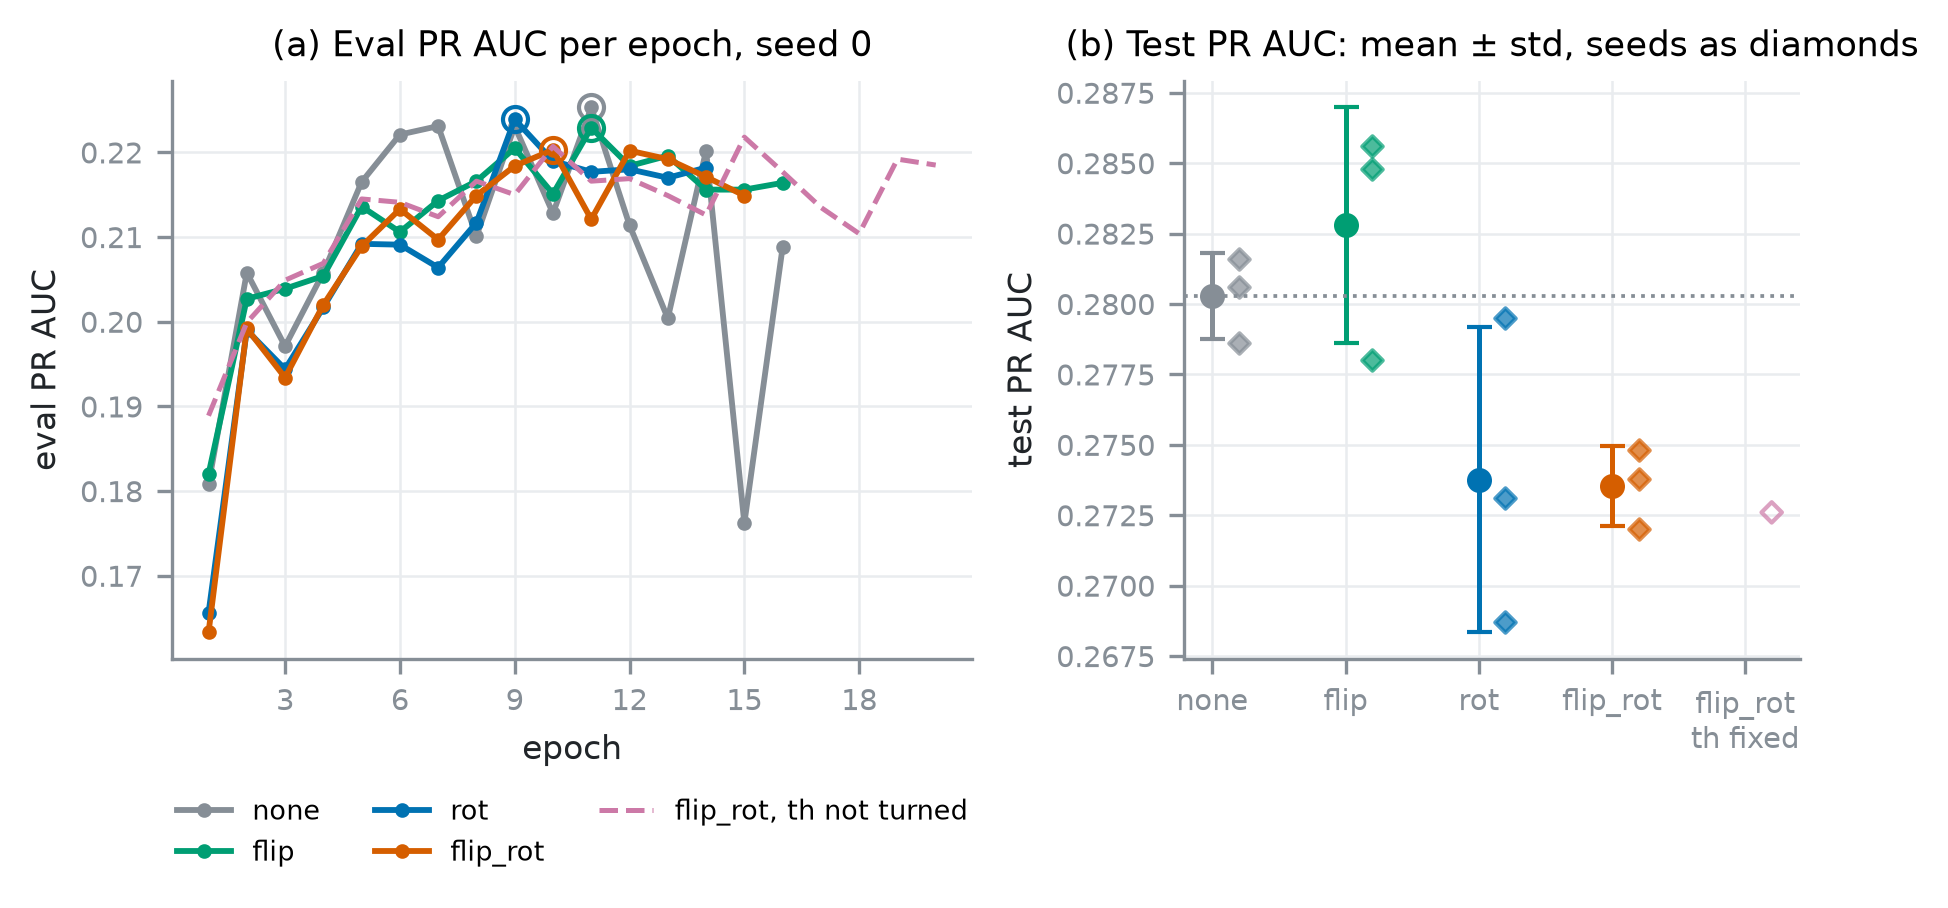
\includegraphics[width=\columnwidth]{dl/figures/aug_ablation.png}
\caption{(a) Eval PR AUC per epoch for seed 0; circles mark the kept epoch. (b) Test PR AUC, mean $\pm$
standard deviation over seeds 0--2, with the single seeds as diamonds; the dotted line is no augmentation.}
\label{fig:dl_aug}
\end{figure}

\textbf{Result.} No augmentation reliably helps (Table~\ref{tab:dl_aug}, Fig.~\ref{fig:dl_aug}). On eval
the modes lie within 0.006 of each other. On test, flips alone are neutral (0.283 $\pm$ 0.004 against
0.280 $\pm$ 0.002), while \texttt{rot} and \texttt{flip\_rot} are lower for each of the three seeds, by
0.006 and 0.007 on average. Paired over the same fire events against the no-augmentation model of the same
seed, every 95\% interval contains zero: the differences range from $-0.012$ ($-0.024$ to 0.002) for
\texttt{rot} with seed 0 to $+0.005$ ($-0.007$ to 0.013) for \texttt{flip} with seed 0. Augmentation also
delays convergence slightly, with the best epoch at 12.3 on average for \texttt{flip\_rot} against 9.3 for
none.

Taken literally, our rule picks \texttt{rot}: its mean eval PR AUC is 0.0042 above none, against a seed
standard deviation of 0.0038. We do not follow it here. A margin of 0.0004 over a standard deviation
estimated from three seeds is not evidence of a gain, and on test \texttt{rot} is lower than none for every
seed. The final U-Net is therefore trained without augmentation; flips alone would be an equally
defensible choice, but they bring no measurable gain.

Turning the wind direction made no measurable difference in the one run that tests it: \texttt{flip\_rot}
scores 0.274 with \texttt{th} turned and 0.273 without (paired difference $+0.001$, $-0.013$ to 0.013).
The U-Net seems to draw little from \texttt{th} in this setting, so this run cannot show how much
wrong wind physics would hurt; the transform is correct by construction and by the self-check above.

Why do rotations not help? The data is not rotation-invariant. The south-up grid fixes north and south,
terrain aspect differs between them, and the fires come with prevailing wind regimes, so a rotated patch
shows combinations that are rare in the test set. The model is also not short of data: its learning curve
is flat beyond half of the training set (Section~\ref{sec:dl_validation}). The baseline itself moved with
the hardware: without augmentation the U-Net scores 0.280 $\pm$ 0.002 on the M3 against 0.275 $\pm$ 0.008
on the T4, which is why every run in this comparison used the same machine.
